\documentclass{article}
\usepackage[utf8]{inputenc}
\usepackage{float}
\usepackage{graphicx}
\usepackage{multirow}
\usepackage{amsmath}
\usepackage{tikz}

\title{Stereo Vision}
\author{Richard Daelan Roosa}
\date{Summer 2020}

\begin{document}
\maketitle

\section{Introduction}
This document seeks to explore the effects of the physical parameters of the stereo camera system, and the physical limitations they impose on any depth-determination algorithm applied to the same.
The most basic stereoscopic camera array (like the ones studied here) consist of a pair of cameras aligned horizontally with a well known horizontal dispacement.
They are aimed such that the central axes of their fields of view are parallel.
This creates a region where the two cameras' respective fields of view overlap; objects in this region appear images produced by both cameras.
Such objects will appear displaced horizontally between the two images.
For example, an object appearing in the center of the image from the camera on the left will appear somewhere to the left of the center of the imgae produced by the camera on the right.
The extent of this "binocular disparity" will be dependent on the distance the object is from the camera array, and can therefore be used to calculate the distance from the camera array to different features common to both images.

\section{Physical Parameters of a Stereoscopic Camera Array}
There are a few important direct physical characteristics of the cameras themselves that impinge heavily on the practical application of such an array.
They are labeled and will be hereafter referred to as follows (see figure \ref{top_down_diag}):

\begin{itemize}
    \item Horizontal and vertical resolution ($r_x$ and $r_y$): the width and height of the image (in pixels). 
    \item Horizontal and vertical field of view ($\Phi_x$ and $\Phi_y$): the angular width and height of the image (in degrees).
    \item Image central axes ($\vec{C_R}$ and $\vec{C_L}$): the axis in each camera bisecting both $\Phi_x$ and $\Phi_y$. $\vec{C_R}$ and $\vec{C_L}$ should be parallel.
    \item Horizontal displacement ($l$): perpendicular distance between $\vec{C_R}$ and $\vec{C_L}$.
\end{itemize}

Camera images are generally presented in as two-dimensional rectangles (for example, on a sheet of 2D paper or a 2D phone/computer screen) and are generally thought of consisting of rectangular pixels.
However, in reality, a camera image is two-dimensional representation of a spherical rectangle,\footnote{A spherical rectangle is a region of the surface of a sphere bounded by two pairs of planes, where each plane passes through the center of the sphere, and the lines of intersection formed by each pair are perpendicular.} of which each pixel is a section, itself a spherical rectangle.
Therefore, the width of a pixel can be used as a unit of angular measurement, where each pixel represents an equal proportion of the total field of view.
The angular width of a pixel in the horizontal dimension ($\phi_x$) is given by its proportion of the total horizontal field of view of the camera.

\begin{equation}
    \phi_x = \frac{\Phi_x}{r_x}
\end{equation}

Therefore, for a standard definition video camera (with a resolution of 640x480 pixels) and a 45$^{\circ}$ horizontal field of view, each pixel represents 0.07$^\circ$ degrees.
An object appearing 100 pixels to the left of the center of the frame lies on a line passing through the camera's focal point, 7$^\circ$ displaced from the central axis of the image.
These types of measurements form the basis of the depth determination algorithm.

\begin{figure}
    \label{fig:top_down_diag}
    \centering
    \begin{tikzpicture}

        \draw[thick, ->] 
            (0, 0) node[anchor=north east] {$\vec{C_L}$} -- (0, 5) ;
        \draw[thick, ->]
            (3, 0) node[anchor=north west] {$\vec{C_R}$} -- (3, 5);

        \draw[loosely dashed]
            (0,0) -- (-5,5)
            (0,0) -- (5, 5)
            (3,0) -- (-2,5)
            (3,0) -- (8,5); 
        
        \draw[thin, <->]
            (-1, 1.25) node[anchor=south] {$\Phi_x$}
            (-1,1)  arc (135:45:1.414);

        \draw[thin, <-]
            (0,-.25) -- (1.25,-.25);
        
        \draw[thin, ->]
            (1.5,0) node[anchor=north] {$l$}
            (1.75,-.25) -- (3,-.25);

        \foreach \x in {-5,-4,-3,-2,-1,0,1,2,3,4,5}
            \draw[thin]
                (\x, 5.05) -- (\x, 5.15);
        ;

        \draw[thin]
            (-5,5.2) arc (180:90:.25) -- (-.25,5.45) arc (270:360:.25) node[anchor=south] {$r_x = 10$}
            arc (180:270:.25) -- (4.75,5.45) arc (90:0:.25); 

        \fill
            (0,0) circle[radius=2pt] 
            (3,0) circle[radius=2pt];

        \draw[dash dot]
            (0,0) -- (1,5);
        
        \draw[thin, <->]
            (0,2) node[anchor=south east] {$\phi_x$} arc (90:78.7:2);


    \end{tikzpicture}

    \caption{Top-down diagram of a stereoscopic camera array.}

\end{figure}

\section{Depth Determination by Binocular Disparity}
Consider figure \ref{fig:dd1}. 
Object A is positioned such that it is within both cameras' fields of view; it will appear in both images.
Also, as described above, based on the pixels in which Object A appears in both images, we can determine $\alpha_L$ and $\alpha_R$
From there, we can determine trigonometrically that

\begin{equation}
    l = d(\tan\alpha_L + \tan\alpha_R)
\end{equation}

and thus

\begin{equation}
    d = \frac{l}{\tan\alpha_L + \tan\alpha_R}
\end{equation}

\begin{figure}
    \label{fig:dd1}

    \centering
    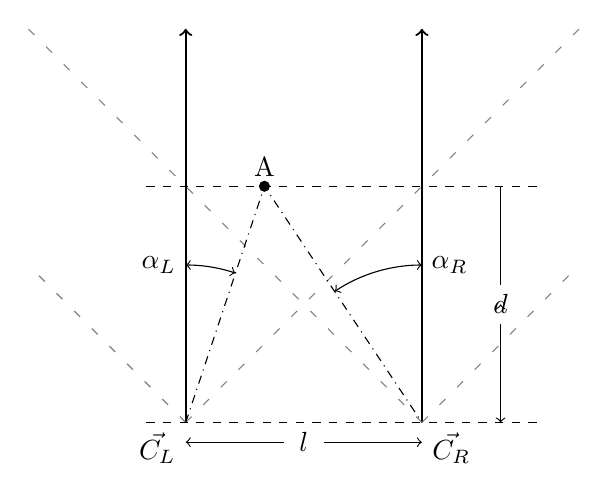
\begin{tikzpicture}


        \draw[thick, ->] 
            (0, 0) node[anchor=north east] {$\vec{C_L}$} -- (0, 5) ;

        \draw[thick, ->]
            (3, 0) node[anchor=north west] {$\vec{C_R}$} -- (3, 5);

        \draw[gray, thin, loosely dashed]
            (0,0) -- (-2,2)
            (0,0) -- (5, 5)
            (3,0) -- (-2,5)
            (3,0) -- (5,2); 
        
        \draw[dashed]
            (-0.5,0) -- (4.5,0)
            (-0.5,3) -- (4.5,3);

        \fill
            (1,3) circle[radius=2pt] node[anchor=south] {A};

        \draw[dash dot]
            (0,0) -- (1,3) -- (3,0);

        \draw[thin, <->]
            (0,2) node[anchor=east] {$\alpha_L$} arc (90:71.6:2);

        \draw[thin, <->]
            (3,2) node[anchor=west] {$\alpha_R$} arc (90:123.6:2);
        
        \draw[thin, ->]
            (4,3) -- (4,1.75) (4,1.5) node {$d$};
        
        \draw[thin, ->]
            (4,1.25) -- (4,0);

        \draw[thin, <-]
            (0,-.25) -- (1.25,-.25);
        
        \draw[thin, ->]
            (1.5,0) node[anchor=north] {$l$}
            (1.75,-.25) -- (3,-.25);


    \end{tikzpicture}
\end{figure}


\section{Accounting for Barrel Distortion}

\end{document}